% !TeX encoding = UTF-8
% !TeX spellcheck = russian-aot
% !TeX program = xelatex
\documentclass[14pt, a4paper, titlepage]{extarticle}

\usepackage[english, main=russian]{babel}
\usepackage{fontspec}
\setmainfont{CMU Serif}
\usepackage[left=30mm, right=15mm, top=20mm, bottom=20mm]{geometry}

\usepackage{microtype}
\usepackage{lettrine}
\renewcommand{\LettrineTextFont}{\upshape}
\usepackage{graphicx}
\usepackage{float}
\usepackage{booktabs}
\usepackage{adjustbox}
\usepackage{comment}

\usepackage{authblk}

\usepackage{csquotes}
\usepackage[left={<<}, right={>>}, leftsub={„}, rightsub={“}]{dirtytalk}
\usepackage[backend=bibtex]{biblatex}
\addbibresource{source.bib}

\linespread{1.3}
\righthyphenmin=2
\parskip=0pt
\parindent=1.25cm

\title{Методы искусственного интеллекта.~Аналитический обзор на~тему <<Модели представления знаний>>, задачи}
\author{В.\,С.\,Верхотуров \\ БСБО-05-20}
\affil{РТУ МИРЭА}

\usepackage{hyperref}
\hypersetup{pdftitle={Методы искусственного интеллекта. Аналитический обзор на тему <<Модели представления знаний>>, задачи}, pdfauthor={В. С. Верхотуров}}

\begin{document}
\maketitle

\section*{Аннотация}
Выбор подходящего метода для представления знаний о реальном мире является одним из основных вопросов, связанных с искусственным интеллектом.\cite{rashid2015semantic}

\section{Основные понятия, используемые в моделях представления знаний~\cite{белоус2010современные}}

Индивид (денотат, объект, экземпляр)~--- существующий в единственном экземпляре представитель своего класса, которому можно присвоить уникальный индекс.

Концепт может быть эксплицитно (перечислением) задан множеством конкретных индивидов или имплицитно (содержательно) определён с помощью описания через другие уже известные концепты.

Свойство (роль, признак, слот)~--- один из атрибутов концепта, характеризующих его с какой-либо точки зрения. Для концептов этот атрибут может иметь имя и не иметь точного значения, но должен иметь область определения значений. Для индивидов свойство имеет точное значение.

Область определения значений свойств (ограничитель, фацет)~--- множество возможных конкретных значений свойства, заданное либо их перечислением, либо пределами значений, либо описанное через другие, уже известные области значений (типы, домены).

Отношение~--- множество пар или троек, или кортежей n-й размерности, задающее свойства концептов и индивидов, проявляемые ими при взаимодействии с другими концептами или индивидами. Принадлежность конкретного кортежа этому множеству говорит о существовании свойств у элементов кортежа, проявляемых в их взаимодействии.

Ситуативная структура (ситуация, сложное отношение, фрейм)~--- система (множество) отношений, определённых на конечном множестве концептов или индивидов, называемых в этом случае <<элементами ситуации>> или <<элементами сложного отношения>>. Ситуативная структура может предполагать существование у ее элементов каких-либо свойств.

\section{Формы представления знаний}

Знания в определённой базе представлены в определённой форме. Форма представления знаний оказывает существенное влияние на характеристики и свойства системы, поэтому представление знаний является одной из наиболее важных проблем, характерных для систем, основанных на знаниях.\cite{белоус2010современные}

Наиболее часто используемые и популярные на сегодняшний день модели представления знаний\cite{карелин2014модели}:
\begin{enumerate}
	\item семантические сети \cite{нильсон1985принципы, попова2019основные, nguyen2020lemma, загорулько2011подход};
	\item концептуальные сети \cite{шенк1980обработка};
	\item ситуационное управление \cite{поспелов2020ситуационное};
	\item логическое представление знаний \cite{братко2004алгоритмы};
	\item фреймы для представления знаний \cite{минский1979фреймы};
	\item растущие пирамидальные сети \cite{гладун2004растущие};
	\item признаковые структуры \cite{knight1989unification};
	\item онтологии для описания семантики \cite{abdul2007common}.
\end{enumerate}



\printbibliography

\clearpage

\section{Задачи}

\subsection{Задача 1. Продукционная модель}

\subsubsection*{Условие}

Построить продукционную модель представления области \say{Продуктовый магазин}.

\subsubsection*{Решение}

\begin{enumerate}
	\item Обязательное действие, выполняемое в продуктовом магазине~--- покупка еды;
	\item прежде чем купить товар, его необходимо взять в упаковке или на развес;
	\item чтобы выбрать, брать ли в упаковке товар или на развес, необходимо сравнить отношение цены к качеству продукта;
	\item прежде чем сравнить товары, необходимо прийти в магазин и подойти к полкам каждого из товаров;
	\item прежде чем пойти в магазин, необходимо иметь при себе деньги и потребность в товаре.
\end{enumerate}

\begin{itemize}
	\item Если у субъекта есть потребность в товаре и деньги, то субъект может пойти в магазин;
	\item если субъект пришел в магазин, то субъект должен подойти к каждой из двух полок с товаром;
	\item если субъект подошёл к полке полке, то субъекту необходимо посчитать отношение цены к качеству товара;
	\item если субъект обошёл все требуемые полки, то ему необходимо принять решение, какой товар брать;
	\item если субъект принял решение, какой товар наиболее выгоден, то его необходимо купить.
\end{itemize}

Введём обозначения для фактов (Ф), действий (Д) и продукций (П), тогда:\\
Субъект = Петр;\\
Ф1=у субъекта есть потребность в продукте;\\
Ф2=у субъекта есть достаточная сумма денег;\\
Ф3=отношение качества товара к его цене на развес больше, чем в упаковке;\\
Д1=субъект может пойти в магазин;\\
Д2=субъект подошёл к полке с товаром в упаковке;\\
Д3=субъект подошёл к полке с товаром на развес;\\
Д4=субъект оценил товары;\\
Д5=субъект взял товар в упаковке;\\
Д6=субъект взял товар на развес;\\
Д7=субъект купил товар;\\

Для продукций установим приоритет (в скобках перед запятой, чем выше приоритет, чем раньше проверяется правило).\\

\begin{tabular}{ll}
	П1(4, Ф1 и Ф2)=Д1 &\\
	П2(3, Д1 и Д2)=Д3, Д4 & П3(3, Д1 и Д3)=Д2, Д4 \\
	П4(2, Д4 и Ф3)=Д6 & П5(2, Д4 и не Ф3)=Д5
	П6(1, Д5 или Д6)=Д7
\end{tabular}

\noindent @startuml\\
usecase "П1(4, Ф1 и Ф2)" as P1\\
usecase "П2(3, Д1 и Д2)" as P2\\
usecase "П3(3, Д1 и Д3)" as P3\\
usecase "П4(2, Д4 и Ф3)" as P4\\
usecase "П5(2, Д4 и не Ф3)" as P5\\
usecase "П6(1, Д5 или Д6)" as P6\\
usecase "Д1" as D1\\
usecase "Д2" as D2\\
usecase "Д3" as D3\\
usecase "Д4" as D4\\
usecase "Д5" as D5\\
usecase "Д6" as D6\\
usecase "Д7" as D7\\
P1 --> D1\\
P2 --> D3\\
P3 --> D4\\
P3 --> D2\\
P2 --> D4\\
P4 --> D6\\
P5 --> D5\\
P6 --> D7\\
D1 --> P2\\
D1 --> P3\\
D3 --> P3\\
D2 --> P2\\
D4 --> P4\\
D4 --> P5\\
D6 --> P6\\
D5 --> P6\\
@enduml

\begin{figure}[H]
	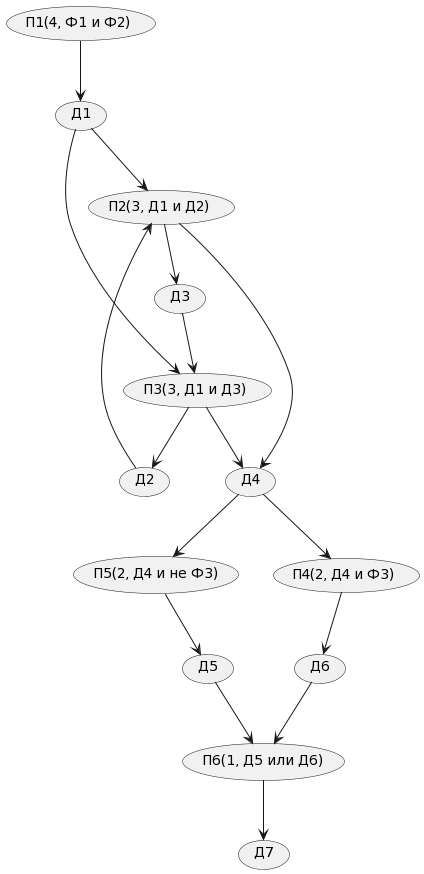
\includegraphics[scale=.8]{pic1}
	\caption{Схема продукций предметной области <<Магазин>>.}
\end{figure}

\subsection{Семантическая сеть}

\subsubsection*{Условие}

Построить сетевую модель представления области \say{Продуктовый магазин}.

\subsubsection*{Решение}

\noindent
@startuml\\
class Человек\\
\\
class Клиент\\
Клиент : Цель\\
Клиент : Деньги\\
\\
class Кассир\\
\\
\\
Клиент --|> Человек\\
Кассир --|> Человек\\
\\
class Продукт\\
Продукт : Цена\\
class Продукт\_на\_развес\\
class Продукт\_в\_упаковке\\
Продукт\_на\_развес --|> Продукт\\
Продукт\_в\_упаковке --|> Продукт\\
\\
class Продуктовый\_магазин\\
object Магазин\_Десяточка\\
Продуктовый\_магазин : Адрес\\
Продуктовый\_магазин : Название\\
Продуктовый\_магазин : [Продукт]\\
\\
object Картошка\_на\_развес\\
object Картошка\_в\_упаковке\\
Продуктовый\_магазин --> Продукт : имеет\\
Магазин\_Десяточка --> Картошка\_на\_развес : имеет\\
Магазин\_Десяточка --> Картошка\_в\_упаковке : имеет\\
object Пётр\\
Клиент -->  Пётр : например\\
Пётр --> Магазин\_Десяточка : пришёл\\
Продукт\_на\_развес --> Картошка\_на\_развес : например\\
Продукт\_в\_упаковке --> Картошка\_в\_упаковке : например\\
\\
Пётр --> Картошка\_на\_развес : оценил\\
Пётр --> Картошка\_в\_упаковке : оценил\\
Пётр --> Картошка\_на\_развес : взял\\
Пётр --> Картошка\_в\_упаковке : взял\\
\\
object Кассир\_Галя\\
Кассир --> Кассир\_Галя : например\\
Пётр --> Кассир\_Галя : расплатился\\
@enduml

\begin{figure}[H]
	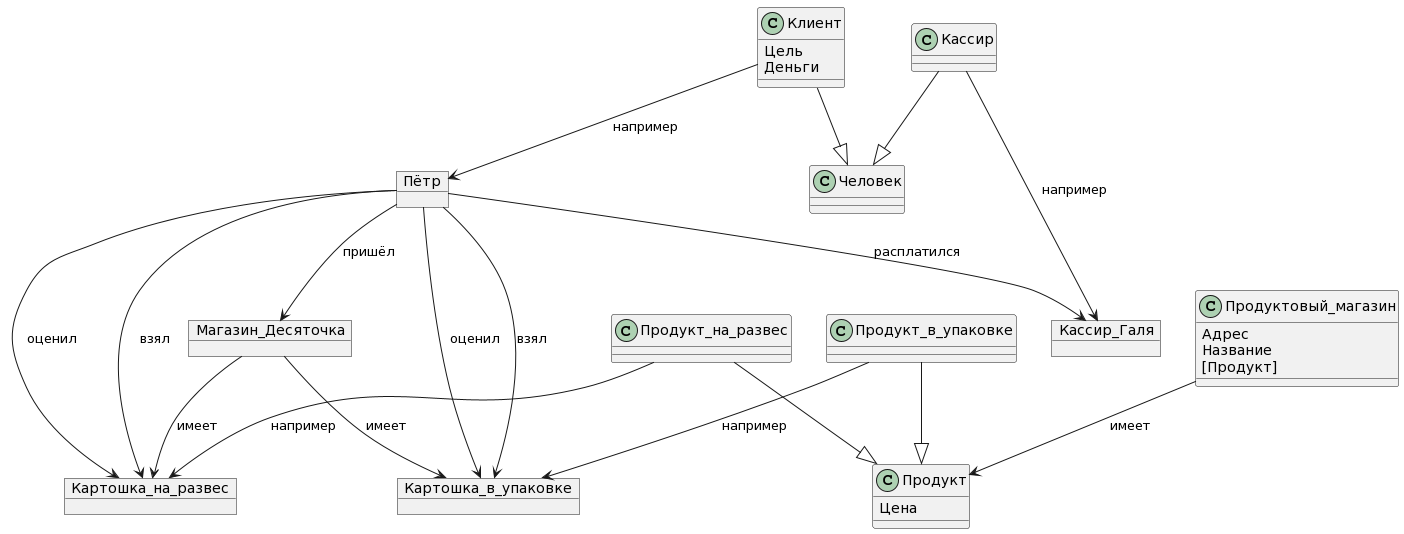
\includegraphics[width=\textwidth]{pic2}
	\caption{Семантическая сеть предметной области <<Магазин>>.}
\end{figure}

\subsection{Фреймовая модель}

\subsubsection*{Условие}

Построить фреймовую модель представления области \say{Продуктовый магазин}.

\subsubsection*{Решение}

\begin{table}[H]
\begin{adjustbox}{width=\columnwidth,center}
\begin{tabular}{cccc}
	\toprule
	\multicolumn{4}{c}{Человек} \\
	\midrule
	Имя слота & Значение слота & Способ получения значения & Демон
	\\\midrule
	
	пол & М или Ж & из внешних источников & \\
	возраст & от 0 до 120 лет & из внешних источников & \\
	
	\bottomrule
\end{tabular}
\end{adjustbox}
\end{table}

\begin{table}[H]
\begin{adjustbox}{width=\columnwidth,center}
\begin{tabular}{cccc}
	\toprule
	\multicolumn{4}{c}{Магазин} \\
	\midrule
	Имя слота & Значение слота & Способ получения значения & Демон
	\\\midrule
	
	Адрес & Город, улица, дом, уточнения & из внешних источников & \\
	Название & & из внешних источников & \\
	Часы работы & & из внешних источников & \\
	\bottomrule
\end{tabular}
\end{adjustbox}
\end{table}

Фреймы-наследники:
\begin{table}[H]
	\begin{adjustbox}{width=\columnwidth,center}
		\begin{tabular}{cccc}
			\toprule
			\multicolumn{4}{c}{Клиент(АКО Человек)} \\
			\midrule
			Имя слота & Значение слота & Способ получения значения & Демон
			\\\midrule
			
			Продуктова корзина & фрейм-ситуация & из внешних источников & \\
			пол & М или Ж & из внешних источников & \\
			возраст & от 0 до 120 лет & из внешних источников & \\
			
			\bottomrule
		\end{tabular}
	\end{adjustbox}
\end{table}

\begin{table}[H]
	\begin{adjustbox}{width=\columnwidth,center}
		\begin{tabular}{cccc}
			\toprule
			\multicolumn{4}{c}{Кассир (АКО Человек)} \\
			\midrule
			Имя слота & Значение слота & Способ получения значения & Демон
			\\\midrule
			
			возраст & от 18 до 55 лет & из внешних источников & \\
			стаж работы & & из внешних источников & \\
			зарплата & & из внешних источников & \\
			график работы & & из внешних источников & \\
			место работы & Магазин Десяточка & из внешних источников & \\
			
			\bottomrule
		\end{tabular}
	\end{adjustbox}
\end{table}

Фреймы-образцы:

\begin{table}[H]
	\begin{adjustbox}{width=\columnwidth,center}
		\begin{tabular}{cccc}
			\toprule
			\multicolumn{4}{c}{Магазин Десяточка (АКО Магазин)} \\
			\midrule
			Адрес & ул. Горького д. 2 пар. 2 & из внешних источников & \\
			Название & Десяточка & из внешних источников & \\
			Часы работы & с 9:00 до 21:00 & из внешних источников & \\
			\bottomrule
		\end{tabular}
	\end{adjustbox}
\end{table}

\begin{table}[H]
	\begin{adjustbox}{width=\columnwidth,center}
		\begin{tabular}{cccc}
			\toprule
			\multicolumn{4}{c}{Пётр (АКО Клиент)} \\
			\midrule
			Имя слота & Значение слота & Способ получения значения & Демон
			\\\midrule
			
			Продуктовая корзина & фрейм-ситуация & из внешних источников & \\
			пол & М & из внешних источников & \\
			возраст & 20 лет & из внешних источников & \\
			\bottomrule
		\end{tabular}
	\end{adjustbox}
\end{table}

\begin{table}[H]
	\begin{adjustbox}{width=\columnwidth,center}
		\begin{tabular}{cccc}
			\toprule
			\multicolumn{4}{c}{Кассир Галина (АКО Кассир)} \\
			\midrule
			Имя слота & Значение слота & Способ получения значения & Демон
			\\\midrule
			
			возраст & 20 лет & из внешних источников & \\
			стаж работы & 1 год & из внешних источников & \\
			зарплата & 30\,000 руб. & из внешних источников & \\
			график работы & День через день с 9:00 до 21:00 & из внешних источников & \\
			место работы & Магазин Десяточка & из внешних источников & \\
			
			\bottomrule
		\end{tabular}
	\end{adjustbox}
\end{table}

Фреймы-ситуации:
\begin{table}[H]
	\begin{adjustbox}{width=\columnwidth,center}
		\begin{tabular}{cccc}
			\toprule
			\multicolumn{4}{c}{Продуктовая корзина} \\
			\midrule
			Имя слота & Значение слота & Способ получения значения & Демон
			\\\midrule
			
			товары & & из внешних источников & IF-ADDED (изменяет слот «Перечень цен», «удовлетворённость клиента товарами») \\
			перечень цен &  & присоединённая процедура & IF-ADDED (изменяет слот «Сумма заказа») \\
			оценка удовлетворённости клиента товарами &  & присоединённая процедура & \\
			сумма заказа & & присоединённая процедура & \\
			дата оплаты & & из внешних источников & \\
			кассир & фрейм-образец & из внешних источников & IF-ADDED (изменяет слот «Дата оплаты»)\\
			
			\bottomrule
		\end{tabular}
	\end{adjustbox}
\end{table}

Фреймы-сценарии:

\begin{table}[H]
	\begin{adjustbox}{width=\columnwidth,center}
		\begin{tabular}{cccc}
			\toprule
			\multicolumn{4}{c}{Посещение продуктового магазина} \\
			\midrule
			Имя слота & Значение слота & Способ получения значения & Демон
			\\\midrule
			
			клиент & фрейм-объект & из внешних источников & \\
			продуктовый магазин & фрейм-объект & из внешних источников & IF-ADDED, IF-REMOVED (изменяют слот «Кассир») \\
			Сцена 1 & Вход, оценка товаров &  & \\
			Сценка 2 & & Оплата & \\
			Сцена 3 & Выход & из внешних источников & \\
			
			\bottomrule
		\end{tabular}
	\end{adjustbox}
\end{table}

\begin{table}[H]
	\begin{adjustbox}{width=\columnwidth,center}
		\begin{tabular}{cccc}
			\toprule
			\multicolumn{4}{c}{Посещение продуктового магазина Десяточка (АКО Посещение продуктового магазина)} \\
			\midrule
			Имя слота & Значение слота & Способ получения значения & Демон
			\\\midrule
			
			клиент & Пётр & из внешних источников & \\
			продуктовый магазин & Магазин Десяточка & из внешних источников & IF-ADDED, IF-REMOVED (изменяют слот «Кассир») \\
			Сцена 1 & Вход, оценка товаров Петра в магазине Десяточка & Кассир Галя & \\
			Сцена 2 & Оплата Петр & & \\
			Сцена 3 & Выход & из внешних источников & \\
			
			\bottomrule
		\end{tabular}
	\end{adjustbox}
\end{table}

\begin{comment}
@startuml
actor Человек
actor Кассир
actor Клиент
Человек -- Кассир : АКО
Человек -- Клиент : АКО

actor Пётр
Клиент -- Пётр : АКО

actor Кассир_Галина
Кассир -- Кассир_Галина : АКО

agent Магазин
agent Магазин_Десяточка
Магазин -- Магазин_Десяточка : АКО

Магазин_Десяточка --> Кассир_Галина : Слот: место работы

agent Продуктовая_корзина
Продуктовая_корзина --> Пётр : Слот: продуктовая корзина

agent Посещение_продуктового_магазина
agent Посещение_продуктового_магазина_Десяточка
Посещение_продуктового_магазина -- Посещение_продуктового_магазина_Десяточка : АКО
Посещение_продуктового_магазина_Десяточка --> Пётр : Слот: магазин
Посещение_продуктового_магазина_Десяточка --> Магазин_Десяточка : Слот: адрес
Посещение_продуктового_магазина_Десяточка --> Кассир_Галина : Слот: кассир
@enduml
\end{comment}

\begin{figure}[H]
	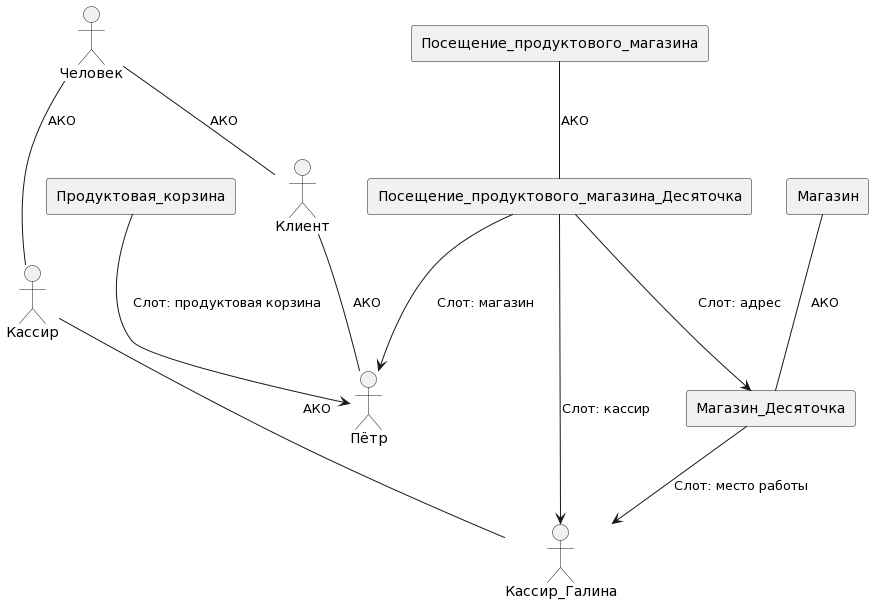
\includegraphics[width=\textwidth]{pic3}
	\caption{Схема фреймов предметной области <<Магазин>>.}
\end{figure}










\end{document}